\documentclass{beamer}
\usepackage{tikz}



\title{VennDiagram presentation}
\author{By: Terry Yi, Kelly Ong, Christopher Zaharia, Micheal O'Malley}


\begin{document}
	
	\frame{\titlepage}
	\begin{frame}[t,label=frameA] {Table of Contents}
		\begin{itemize}
			\item{When to Use Venn Diagrams}
			\item{How to Build Venn Diagrams}
			\item{How to label Venn Diagrams}
		\end{itemize}
	\end{frame}
	%Chris Page 1
	\begin{frame}[t,label=frameA]{When to use Venn Diagrams}
		\begin{itemize}
			\item {We can visually represent differences and similarities between two concepts}
			\item {Used to visualize the logical relationships between sets and their elements}
			\item {Showing the interactions between different sets of data, such as the overlap or intersection between two or more sets}
			\item {To visualize the results of a survey or study, showing the distribution of responses across different categories}
			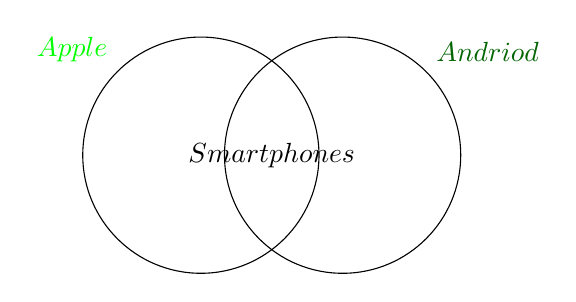
\begin{tikzpicture}
				\node [draw,
				circle,
				minimum size =3cm,
				label={[text={rgb,255:red,0;green,255;blue,0}]135:$Apple$}] (A) at (0,0){};
				
				\node [draw,
				circle,
				minimum size =3cm,
				label={[text={rgb,255:red,0;green,100;blue,0}]45:$Andriod$}] (B) at (1.8,0){};
				
				\node at (0.9,0) {$Smartphones$};	
			\end{tikzpicture}
		\end{itemize}
	\end{frame}
	%Chris Page 2
	\begin{frame}[t,label=frameA]{When to use Venn Diagrams}
		\begin{itemize}
			\item {Demonstration of the different components of a larger system, showing how each component relates to the others}
			\item {The aid in understanding the concepts of union, intersection, and complement in set theory}
			\item {Demonstration of the hierarchy of a system, showing how different levels of the system are related to each other}
			\item {To provide a clear and concise visual summary of complex information, making it easier for the audience to understand and remember}
		\end{itemize}
	\end{frame}
	
	\begin{frame}[t,label=frameA]{How to Build a Venn Diagram}
		\begin{itemize}
			\item{\textbf{1. Use the "tikz" package}}
			\item{The "tikz" package is a tool used to create graphic elements in LaTeX}
			\item{At the beginning of your document, import the tikz package with " \textbackslash usepackage\{tikz\} "}
			%			\begin{figure}[h]
				%				\includegraphics[scale=.6]{venn-diagram-code.jpg}
				%				\caption{This is the code to create a Venn Diagram in Latex}
				%			\end{figure}
		\end{itemize}
	\end{frame}
	
	\begin{frame}[t,label=frameA]{How to Build a Venn Diagram}
		\begin{itemize}
			\item{\textbf{2. How to draw the first circle}}
			\item{INSERT HOW TO DRAW FIRST CIRCLE INSTRUCTIONS}
		\end{itemize}
	\end{frame}
	
	\begin{frame}[t,label=frameA]{How to Build a Venn Diagram}
		\begin{itemize}
			\item{\textbf{3. How to create "Intersection"}}
			\item{INSERT INSTRUCTIONS ON HOW TO CREATE INTERSECTION}
		\end{itemize}
	\end{frame}
	
	\begin{frame}[t,label=frameA] {Complete Venn Diagram}
		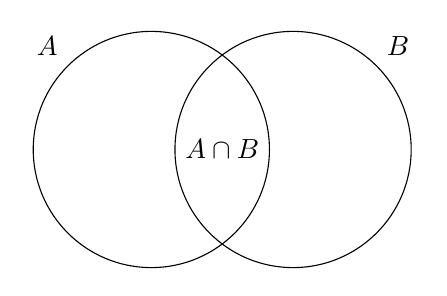
\begin{tikzpicture}
			\node [draw,
			circle,
			minimum size =3cm,
			label={135:$A$}] (A) at (0,0){};
			
			% Set B
			\node [draw,
			circle,
			minimum size =3cm,
			label={45:$B$}] (B) at (1.8,0){};
			
			% Set intersection label
			\node at (0.9,0) {$A\cap B$};
			
		\end{tikzpicture}
	\end{frame}
	%	Mike Page 1
	\begin{frame}[t,label=frameA]{How to Label Venn Diagrams}
		\begin{itemize}
			\item {A Venn Diagram won't be of much use unless there are labels to illustrate what each section of the diagram represents.}
			\item {In the TikZ package, we accomplish this by customizing the individual circles that make up the Venn Diagram. there are several optional arguments in the circle drawing command which can be used to electively color the circle and add a customizable text label.}
			\item {Using optional arguments within this optional argument, we can customize this label's text, position relative to the circle, font size, and font color.}
		\end{itemize}
		
	\end{frame}
	
	
	%	Mike Page 2
	\begin{frame}[t, label=frameA]{Venn Diagram Color and Text Labels}
		\begin{itemize}
			\item{The 'fill' argument in the node command can be used to pick a color for the diagram.}
			\item{For example, "fill=green!50," will result in a green circle that is 50\% transparent.}
			\item{The 'label' argument can be used for a text label.}
			\item{For example, "label=Green Diagram" will result in a label reading "Green Diagram"}
			\item{\tiny"\textbackslash node[draw, circle, minimum size = 3cm, fill = green!50, label=Green Diagram] (greenDiagram) at (0,0)" \large results in the following diagram:}
		\end{itemize}
		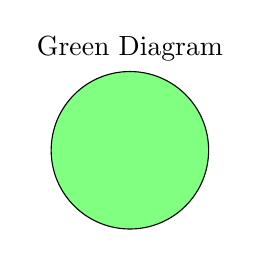
\begin{tikzpicture}
			\node[draw, circle, minimum size = 2cm, fill = green!50, label=Green Diagram] (greenDiagram) at (3,0){};
		\end{tikzpicture}
	\end{frame}
	
	
	%	Mike Page 3
	\begin{frame}[t, label=frameA]{Label Position, Distance, Font Color, and Font Size}
		\begin{itemize}
			\item{The optional 'label' argument has optional arguments of its own, these being label distance, font size, and font color.}
			\item{Label position is determined in relation to a horizontal line through the circle's center. For example, a value of 45 would place the label to 45 degrees, or the top left, of the circle.}
			\item{The 'distance' argument determines how far away from the circle the label is.}
			\item{The 'font color' and 'font size' arguments alter the color and size of the label's text.}
			\item{\tiny "\textbackslash{}node[draw, circle, minimum size = 2cm, fill=purple!75, label=\{[label distance=0.5cm,font=\textbackslash{}large, red]225:A\}] (circleA) at (0,0)\{\};" \\
				"\textbackslash{}node[draw, circle, minimum size = 2cm, fill=cyan!25, label=\{[label distance=0cm,font=\textbackslash{}tiny,
				gray]45:B\}] (circleB) at (5,0)\{\};" \large result in the following:}
		\end{itemize}
		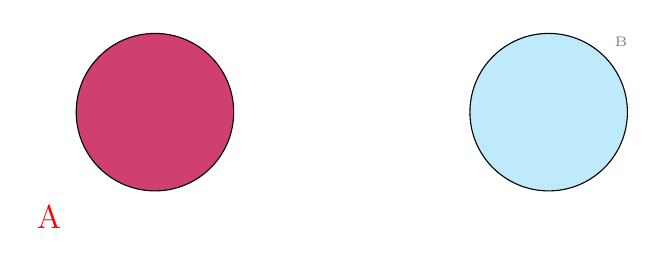
\begin{tikzpicture}
			\node[draw, circle, minimum size = 2cm, fill=purple!75, label={[label distance=0.5cm,font=\large, red]225:A}] (circleA) at (0,0){};
			\node[draw, circle, minimum size = 2cm, fill=cyan!25, label={[label distance=0cm,font=\tiny,
			 gray]45:B}] (circleB) at (5,0){};
		\end{tikzpicture}
	\end{frame}
	
	
	%Mike Page 4
	\begin{frame}[t,label=frameA]{Filling and Labeling Intersections}
	\begin{itemize}
		\item {We color and label intersections in the same way that we label and color individual circles.}
	\end{itemize}
		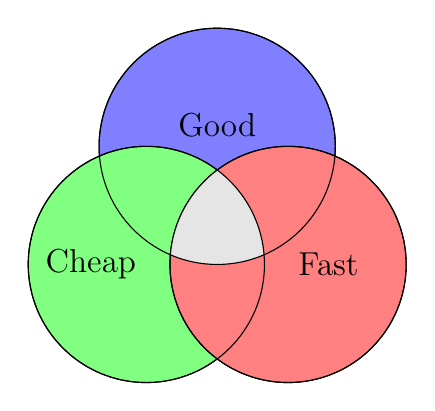
\begin{tikzpicture}
			\node[draw,
			circle,
			minimum size =3cm,
			fill=blue!50,
			label={[label distance=-1.5cm, font=\large]:Good}] (Good) at (0.9,1.5){};
			
			\node[draw,
			circle,
			minimum size =3cm,
			fill=green!50,
			label={[label distance=-1.5cm,font=\large]180:Cheap}] (Cheap) at (0,0){};
			
			\node[draw,
			circle,
			minimum size =3cm,
			fill=red!50,
			label={[label distance=-1.5cm,font=\large]360:Fast}] (Fast) at (1.8,0){};

			%Intersection
			\begin{scope}
				\clip (0,0) circle(1.5cm);
				\clip (1.8,0) circle(1.5cm);
				\clip (0.9,1.5) circle(1.5cm);
				\fill[gray!20](0,0) circle(1.5cm);

			\end{scope}

			%outline
			\draw (0,0) circle(1.5cm);
			\draw (1.8,0) circle(1.5cm);
			\draw (0.9,1.5) circle(1.5cm);
		\end{tikzpicture}

	\end{frame}
	
	
	
	
\end{document}
%Link for basically everything we need :)
%https://latexdraw.com/how-to-draw-venn-diagrams-in-latex/
